% REFER TO Dr. Dahl's slides.
% Also remember to insert BYU LOGO and 
% the .png.

\documentclass{beamer}
\usepackage{graphicx}
\usepackage{textpos}

\title%[Introduction to Welch's 1938 Paper]
{
       Introduction to Welch's 1938 Paper
}
\logo{%
  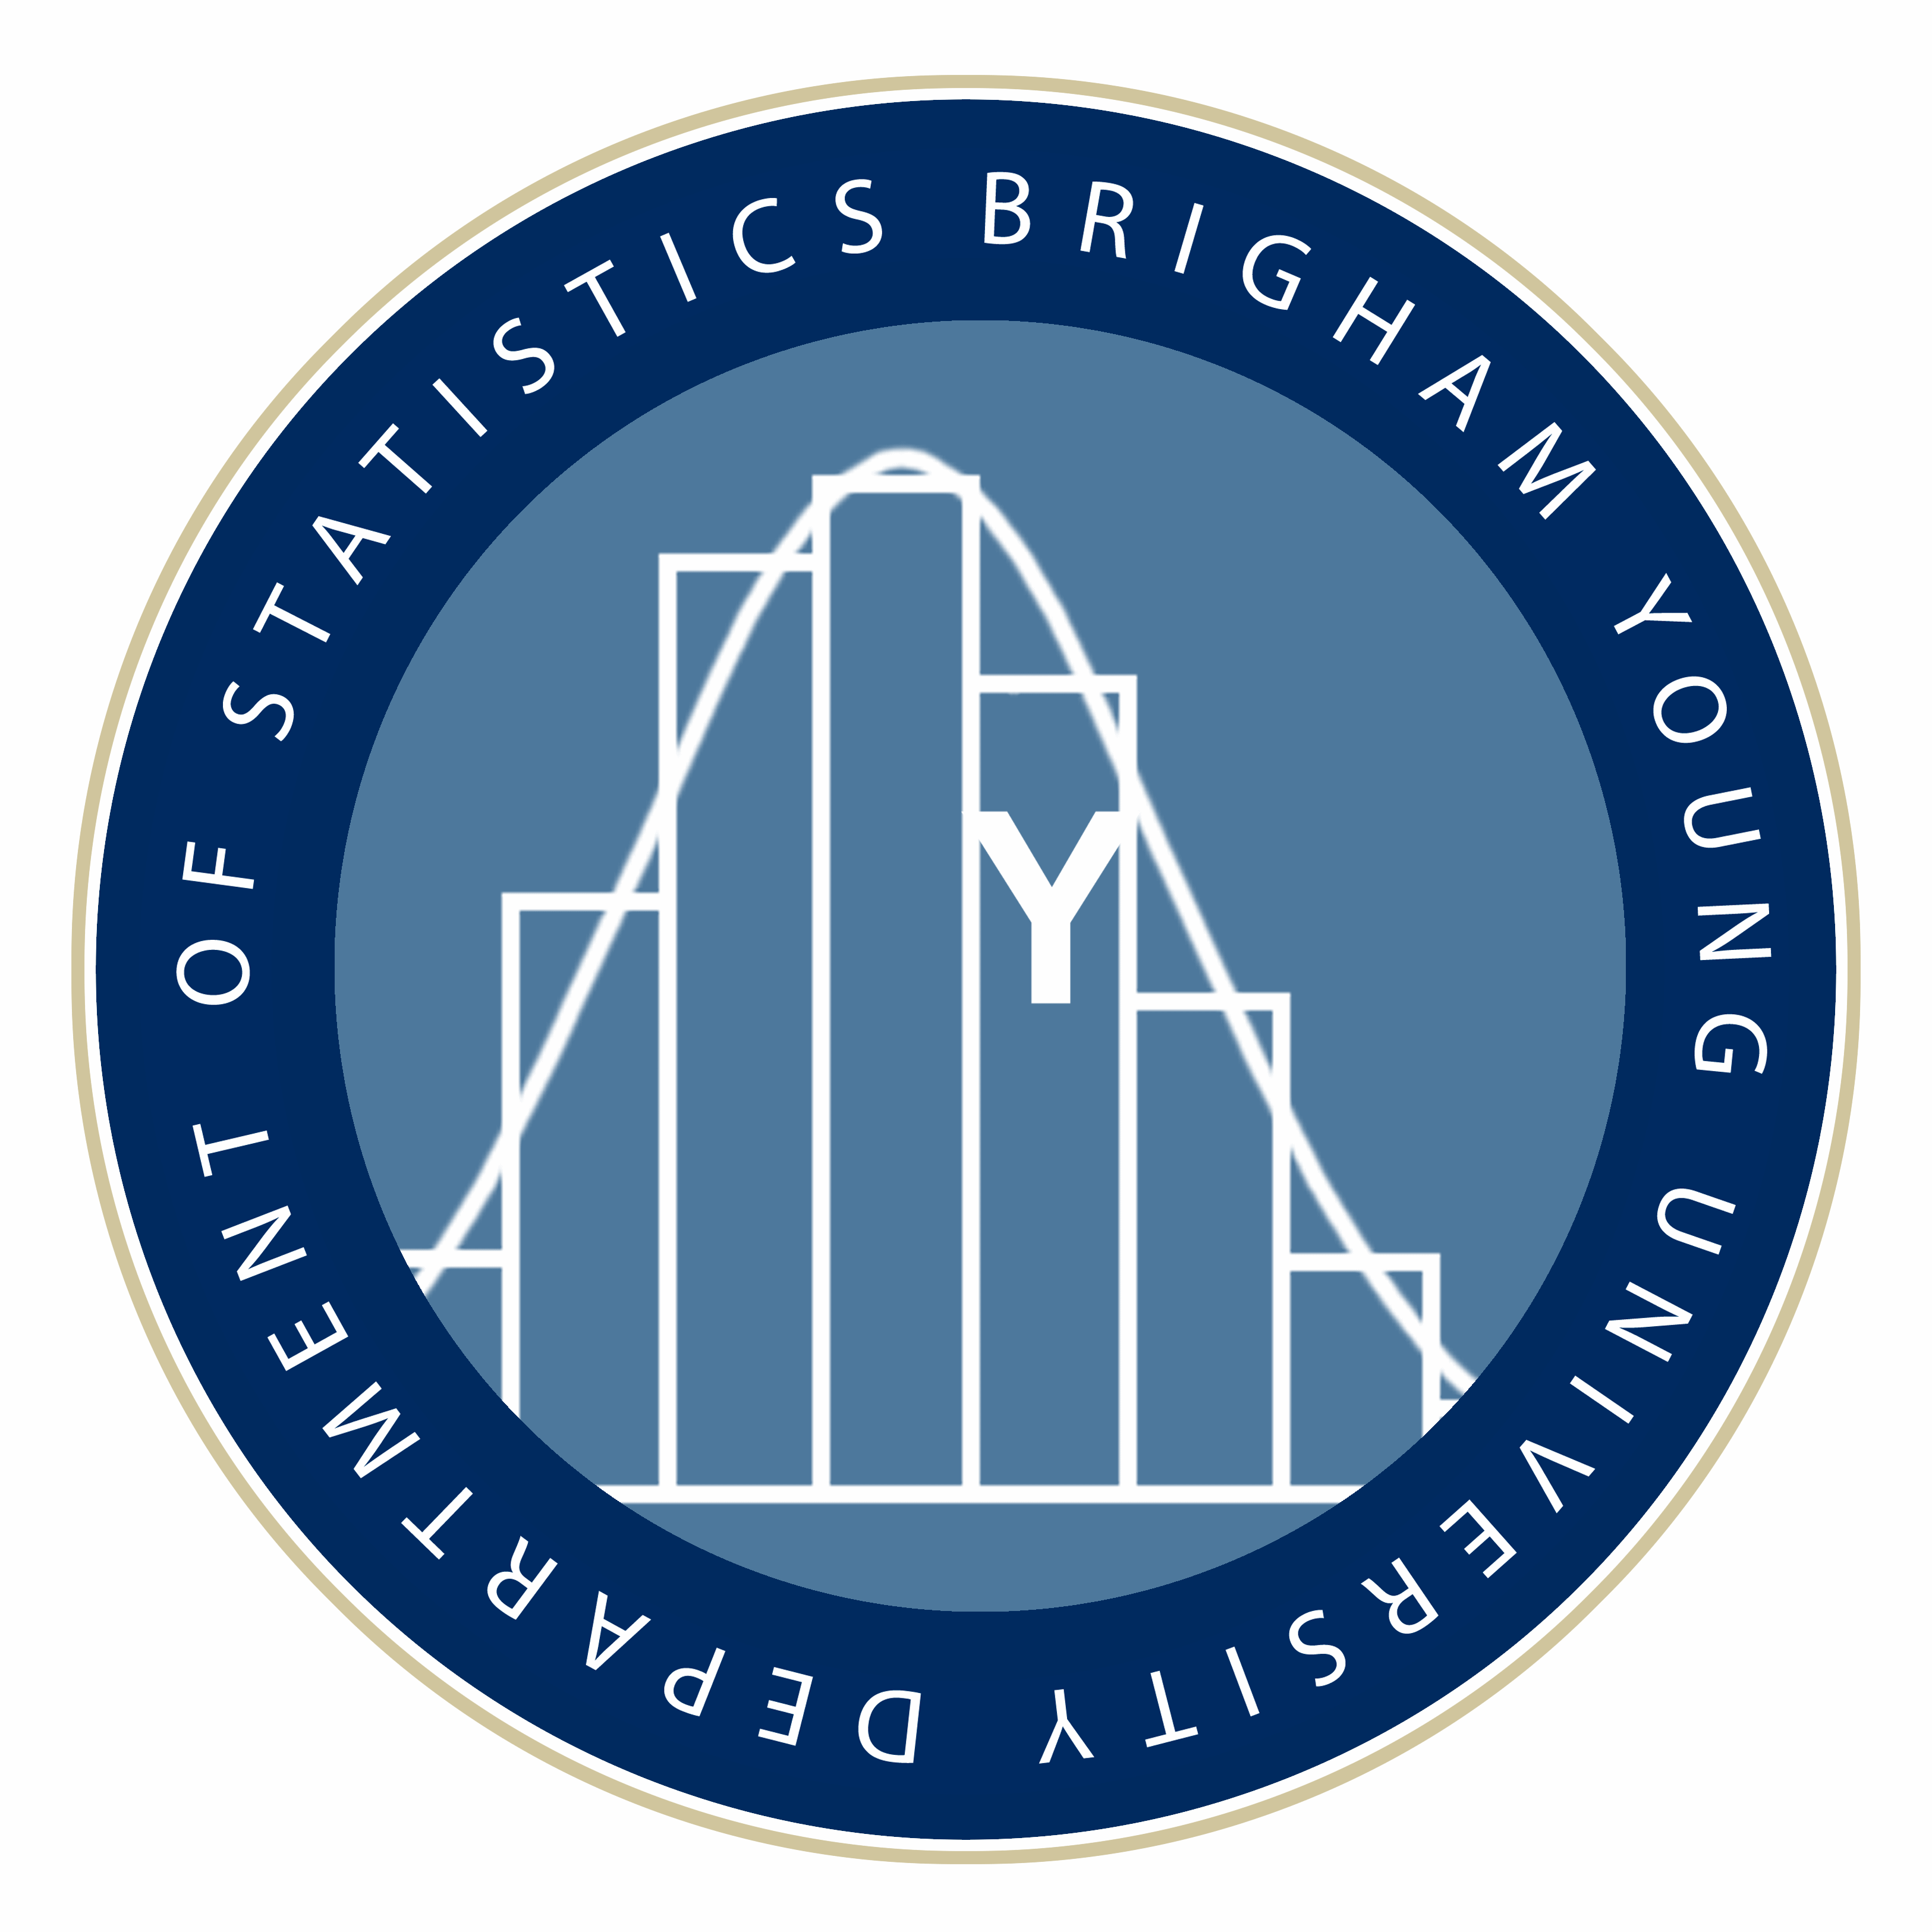
\includegraphics[width=1cm,height=1cm,keepspectration]{logo.png}
}
\usepackage{beamerthemeMadrid}
\author[Arthur Lui]{Arthur L. Lui\inst{1}}

\institute[Brigham Young University]{
  \inst{1}
  Department of Statistics\\
  Brigham Young University
}

\begin{document}

  \begin{frame}
    \titlepage
  \end{frame}

  \begin{frame}
  \frametitle{Part One}
    This is REALLY REALLY AWESOME!
    Suppose that we have samples of sizes $n_1$ and $n_2$ from 
    populations $\pi_1$ and $\pi_2$ respectively. Let the populations be normal in
    form, $\pi_1$ having mean and standard deviation $\alpha_1$ and $\sigma_1$, and
    $\pi_2$ having mean and standard deviation $\alpha_2$ and $\sigma_2$. 
    Let it be required to test whether $\alpha_1$ = $\alpha_2$.  
    Two cases may be distinguished: (i) $\sigma_1$ and $\sigma_2$ may be equal 
    or (ii) they may be unequal. In the first case the most appropriate test 
    for the equality of the $\alpha$'s is made by referring the criterion
    \begin{equation}
      u = \frac{\bar{x_1}-\bar{x_2}}
      {\sqrt{\frac{\Sigma_1+\Sigma_2}{(n_1+n_2-2)}
      \left(\frac{1}{n_1}+\frac{1}{n_2}\right)}}
    \end{equation}
    to the $t$ distribution with $f=(n_1+n_2-2)$.
  \end{frame}

  \begin{frame}
  \frametitle{Part Two}
    In the second case, if the ratio of the two $\sigma$'s is known, 
    a similar criterion can be used: if, however, this ratio is unknown,
    no criterion quite so simple is available. A solution of the problem
    of testing the hypothesis in this instance has been proposed by R. A. Fisher,
    using the concept of fiducial distributions. Fisher notes the equivalence of his
    test to that given previously by W. V. Behrens in 1929. the validity of this
    test has, however, been questioned by M. S. Barlett. An alternative criterion
    which has been often employed is
    \begin{equation}
    v = \frac{\bar{x_1}-\bar{x_2}}
    {\sqrt{\frac{\Sigma_1}{n_1(n_1-1)}+\frac{\Sigma_2}{n_2(n_2-1)}}}.
    \end{equation}
    This may be referred to the normal probability table if the samples are large
    enough, but for small samples it does not yield an exact test and it is not
    clear how it may best be made to furnish approximations.
  \end{frame}

  \begin{frame}
  \frametitle{Part Three}
    \begin{center}
      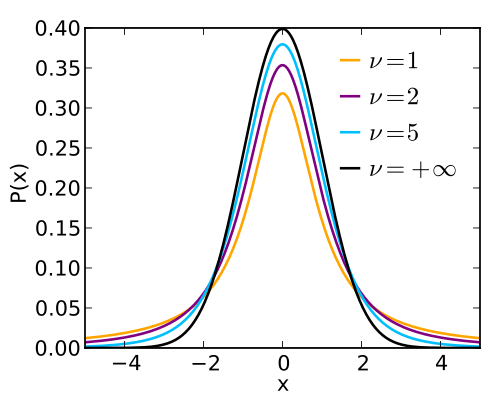
\includegraphics[scale=.25]{tDist.png} 
    \end{center}
    It is easily seen that $u$ in general is not distributed as $t$. For whereas the
    square of the standard error of $(\bar{x_1}-\bar{x_2})$ is
    $(\sigma_1^2/n1+\sigma_2^2/n2)$, the quantity under the root in (1) is an
    unbiased estimate of
    \[
    \frac{(n_1-1)\sigma_1^2+(n_2-1)\sigma_2^2}{n_1+n_2-2}
    \left(\frac{1}{n_1}+\frac{1}{n_2}\right).
    \]
  \end{frame}  

  \begin{frame}
  \frametitle{The End}
    That's it! Thanks for listening! 
  \end{frame}
\end{document}
